\newpage
\section{Билет 19. Постановка задач теории упругости в перемещениях и напряжениях. Граничные условия. Принцип Сен-Венана.}

\subsection{В перемещениях}
Если на границе тела заданы перемещения, удобно в качестве основных уравнений брать уравнения теории упругости в перемещениях, которые называются уравнениями Навье-Ламе. Они получаются из общих уравнений количества движения с использованием закона Гука и формул, выражающих компоненты тензора деформации через перемещения. Уравнения Навье-Ламе выглядят следующим образом:
$$
\rho_0\frac{\partial^2 w^i}{\partial t^2} = \rho_0 F^i + (\lambda + \mu)g^{ij}\nabla_j \mathrm{div} \vec{w} + \mu \Delta w^i
$$

Если на поверхности тела заданы перемещения, то из уравнений Навье-Ламе определяется вектор $w$ и этим решается задача о равновесии упругого тела в перемещениях. Напряжения при этом могут быть найдены согласно закону Гука. 

\subsection{В напряжениях}

При решении задачи в напряжениях, используются уравнения равновесия в напряжениях  $$\rho_0 F^i + \nabla_j p^{ij} = 0$$, эти три уравнения содержат шесть неизвестных компонент тензора напряжений и составляют незамкнутую систему. В некоторых случаях, например из симметрии задачи, можно заранее понять, что в эти уравнения входят только три неизвестные компоненты напряжений и если на границе известны $p_n$, то можно найти напряжения используя только эти три уравнения.

В общем случае, с помощью закона Гука из уравнений совместности деформаций можно получить дополнительные уравнения, которым должны удовлетворять компоненты тензора напряжений. Эти уравнения называются уравнениями Бельтрами-Мичелла, и выглядят следующим образом:
$$
\Delta p_{ij} + \frac{1}{1+\sigma} \frac{\partial^2 \wp}{\partial x^i \partial x^j}
$$
Причем в декартовых координатах $\wp = p_{11} + p_{22} + p_{33}$.

\newpage
\subsection{Граничные условия}

Граничные условия в задачах теории упругости бывают трёх оснонвх типов:
\begin{enumerate}
\item Граничные условия первого рода: задан вектор $\vec{w}$ на всей поверхности тела $\Sigma$
\begin{center}
$\vec{w}\mid_{\Sigma} = \vec{f}(x^i,t)$, где $\vec{f}$ - заданная функция
\end{center}

\item Граничные условия второго рода: на поверхности тела $\Sigma$ задан вектор напряжений $\vec{P_n}$ как функция времени и координат точек поверхности
\begin{center}
$\vec{P_n}\mid_{\Sigma} = \vec{\varphi}(x^i,t)$, где $\vec{\varphi}$ - заданная функция
\end{center}

\item Граничные условия третьего рода: на одной части поверхности тела  $\Sigma_w$ задан вектор $\vec{w}$, а на другой части  $\Sigma_p$ - $\vec{P_n}$
\begin{center}
$\vec{w}\mid_{\Sigma_w} = \vec{f}$ \ \ \ \ \  $\vec{P_n}\mid_{\Sigma_p} = \vec{\varphi}$
\end{center}
\end{enumerate}

\subsection{Принцип Сен-Венана}

\begin{wrapfigure}{R}{0.4\textwidth}
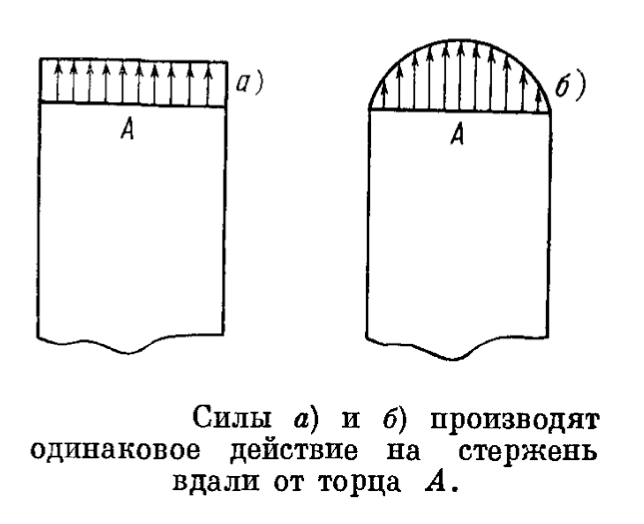
\includegraphics[width=0.4\textwidth]{19/sen_venan.png}
\end{wrapfigure}

Если в некоторой области внутри или на поверхности тела, малой по сравнению с основными размерами тела, на него действует система массовых или поверхностных сил и тело находится в равновесии, то в областях, удаленных от места приложения этих сил, деформированное и напряженное состояния определяются в основном только главным вектором и главным моментом этих сил и приближенно не зависят от детального характера распределения сил. Влияние деталей распределения сил практически сказывается только в непосредственной окрестности области их приложения.
